\documentclass{article}

% Language setting
% Replace `english' with e.g. `spanish' to change the document language
\usepackage[french]{babel}
\usepackage[T1]{fontenc}

% Set page size and margins
% Replace `letterpaper' with `a4paper' for UK/EU standard size
\usepackage[a4paper,top=2cm,bottom=2cm,left=3cm,right=3cm,marginparwidth=1.75cm]{geometry}

% Useful packages
\usepackage{amsmath}
\usepackage{graphicx}
\usepackage[colorlinks=true, allcolors=blue]{hyperref}
\usepackage{minted}
\usepackage{forest}

\title{Projet en informatique pour les sciences humaines}
\author{Johan Cuda}

\begin{document}
\maketitle

\begin{abstract}
Ce projet reprend le travail de threading des widgets de Orange Textable effectué par Antonin Schnyder en proposant de remonter l'architecture de threading d'un étage dans la hiérarchie de classes de Textable. 
\end{abstract}

\tableofcontents

\section{Introduction}

\subsection{Contexte}

\href{http://textable.io/}{Textable} est un add-on du logiciel \href{https://orangedatamining.com/}{Orange} qui permet d'analyser des textes de manière visuelle \footnote{Xanthos, Aris (2014). Textable: programmation visuelle pour l’analyse de données textuelles. In Actes des 12èmes Journées internationales d’analyse statistique des données textuelles (JADT 2014), pp. 691-703. \href{http://lexicometrica.univ-paris3.fr/jadt/jadt2014/01-ACTES/57-JADT2014.pdf}{Read online}}. Textable est composé de widgets développés en Python et qui ont récemment été modifiés par Antonin Schnyder pour optimiser leur processus. En effet, l'interface des widgets se bloque pendant les traitements de données conséquents et leurs performances peuvent être optimisées, c'est pourquoi Antonin Schnyder a modifié ces widgets pour ajouter une logique de \textit{threading} \footnote{À ce sujet voir \href{https://realpython.com/intro-to-python-threading/}{An Intro to Threading in Python}.} qui suit les recommandations de Orange \footnote{Le tutoriel de Orange à ce propos est disponible \href{https://orange3.readthedocs.io/projects/orange-development/en/latest/tutorial-responsive-gui.html}{ici}.}.\newline

Dans ce travail, nous proposons de partir du travail effectué par Antonin Schnyder en remontant d'un étage – dans la hiérarchie de classes de Textable – la logique de threading. Nous avons identifié qu'une grande partie du code qui permet la mise en place du threading se répète dans les widgets, nous avons donc modifié  leur architecture pour faire en sorte que les éléments liés au \textit{threading} soient hérités au travers de la super-classe \textbf{OWTaxtableBaseWidget}.
\newline

Nous commencerons par discuter rapidement de ce qu'est le \textit{threading} puis par expliciter la structure du add-on \textit{Textable} ainsi que d'un widget typique pour mieux comprendre leur fonctionnement. Ensuite, nous listerons les éléments que nous avons identifiés comme possiblement remontables, en mentionnant ceux qui ont directement pu être remonter et en décrivant les modifications effectuées sur ceux qui ne le pouvaient pas. Nous discuterons alors des divers problèmes rencontrés pendant l'implémentation. Finalement, Nous continuerons ce rapport en proposant un tutoriel de développement de widgets qui permet d'exploiter cette nouvelle architecture ainsi que d'assurer en partie l'uniformité des futures widgets qui seront ajoutés à \textit{Textable}. Ce tutoriel reprendra en partie le \href{https://docs.google.com/document/d/1QtXm2aYMZXAyM7mfBTqxt_XrTNFqC7e3aqy7OC1A_18/edit}{tutoriel fourni par Antonin Schnyder}.

\subsection{Qu'est-ce que le threading?}

Ce projet n'a pas pour but d'expliquer ce qu'est le \textit{threading} mais il est quand même nécessaire de fournir une explication succincte du concept pour mieux appréhender le travail proposé dans ce rapport.
L'idée est de répartir le travail entre différent \textit{threads} et de simuler une forme de \textit{multiprocessing}\footnote{Sur la différence entre m\textit{multiprocessing} et \textit{multithreading} voir \href{https://www.geeksforgeeks.org/difference-between-multithreading-vs-multiprocessing-in-python/}{ce lien}.}. À la création de chaque widget, un \textit{main thread} est créé et s'occupera de différents \textit{worker threads} qui seront créés par chaque widget. Le \textit{multithreading} consiste ensuite à faire s'enchaîner l'exécution des \textit{worker threads} pour simuler une sorte de parallélisme des processus. 
Ce système permet donc d'améliorer les performances d'un \textit{software} mais aussi dans notre cas précis de permettre à l'\textit{User interface} (UI) de notre widget de ne pas se bloquer pendant ces calculs. Ceci est extrêmement utile en considérant que suivant la taille des corpus analysés avec \textit{Textable}, les calculs peuvent prendre plusieurs minutes, il est donc pratique de pouvoir annuler le processus en cours grâce au bouton \texttt{Cancel} par exemple.

\section{Structure de \textit{Textable} et des widgets}

\subsection{Structure de \texttt{TextableUtils.py} et \textbf{OWTextableBaseWidget}}

\textit{Textable} peut être visulisé de la manière suivante :
\vspace{5mm}

\fbox{%
\begin{forest}
for tree={
    font=\ttfamily,
    grow'=0,
    child anchor=west,
    parent anchor=south,
    anchor=west,
    calign=first,
    edge path={
        \noexpand\path [draw, \forestoption{edge}]
        (!u.south west) +(5pt,0) |- (.child anchor)\forestoption{edge label};
    },
    inner sep=1pt,
    l=1cm,
    s sep=2mm,
    edge+={darkgray, line width=0.5pt},
    if level=0{
        align=center,
    }{%
        if level=1{font=\bfseries}{}% folder level
    },
    fit=band,
    before typesetting nodes={
        if n=1
            {insert before={[,phantom]}}
            {}
    },
    before computing xy={l=15pt},
}
[\_textable
    [\_\_init\_\_.py]
    [\_\_pycache\_\_]
    [widgets
        [\_\_init\_\_.py]
        [\_\_pycache\_\_]
        [icons]
        [OWTextableCategory.py]
        [...]
        [TextableUtils.py]
    ]
]
\end{forest}
}
\vspace{5mm}

Pour bien comprendre la structure de \textit{Textable} nous allons commencer par considérer le script \texttt{TextableUtils.py} (voir Figure \ref{fig:textable_utils}). Celui-ci contient plusieurs classes qui définissent des éléments utilisables par tous les widgets comme \texttt{InfoBox} ou \texttt{SendButton}. La classe qui nous intéressera le plus sera bien entendu \textbf{OWTextableBaseWidget} : elle est déjà héritée par tous les widgets de \textit{Textable} et a donc été rapidement identifiée comme la classe qui recevrait les modifications relatives au \textit{threading}.

\vspace{5mm}

\begin{figure}[htbp]
    \centering
    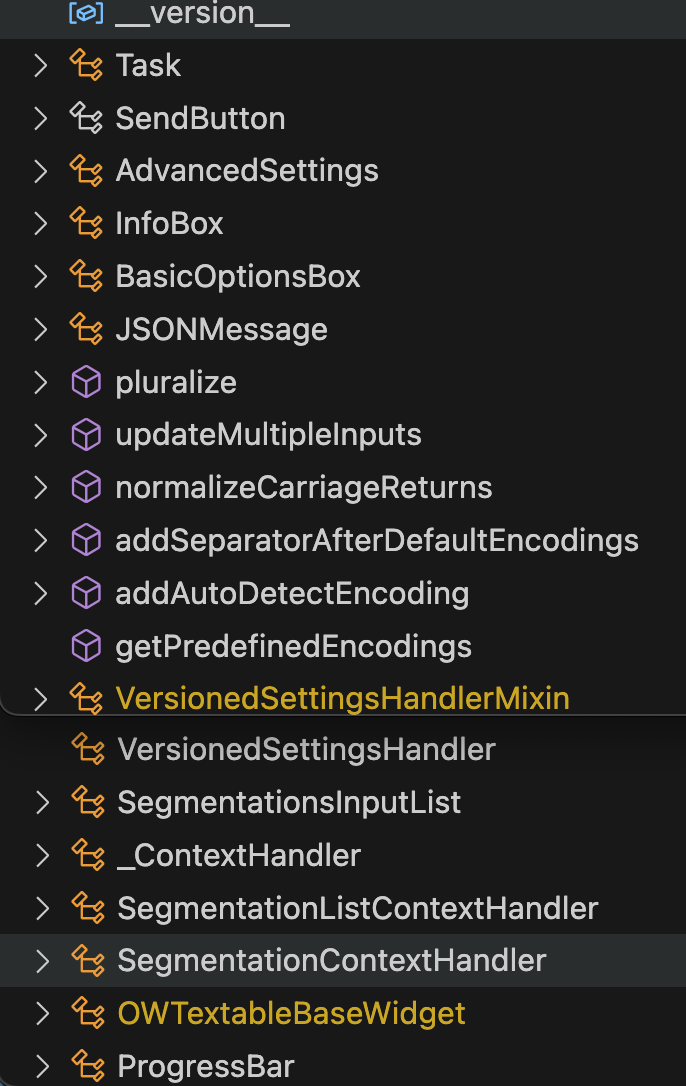
\includegraphics[width=0.25\textwidth]{structure_utils.png}
    \caption{Structure de \texttt{TextableUtils.py}}
    \label{fig:textable_utils}
\end{figure}

\subsection{Structure d'un widget type}

Les widgets ont quand à eu une structure assez uniforme et représentent chacun une classe spécifique qui hérite de la classe \textbf{OWTextableBaseWidget} (par exemple chaque widget \texttt{Count} est une instance de la classe \textbf{OWTextableCount}). Ils sont toujours formés des éléments suivants : 

\begin{enumerate}
    \item Imports divers
    \item Déclaration d'une série d'\textit{attributs de classes}
    \item Déclaration, dans le constructeur de la classe, de tous les \textit{attributs d'instance} ainsi que des éléments d'interface du widget
    \item Déclaration des diverses méthodes propres au processus du widget
\end{enumerate}

La structure générale peut varier selon les widgets mais nous avons ici les éléments principaux.

\section{Analyse des widgets et implémentation}

Nous avons commencé – sur recommandation d'Aris Xantos – par analyser les deux widgets \texttt{Count} et \texttt{Preprocess} car ils sont assez représentatifs de deux types de widgets courants dans \textit{Textable}. Nous avons donc systématiquement repérés tous les éléments liés au \textit{threading} pour ensuite évaluer s'ils étaient remontables dans la classe parente \textbf{OWTextableBaseWidget} ou non. Dans la suite de cette section, nous adopterons les convention suivantes : 

\begin{itemize}
    \item \texttt{Nom\_Du\_Widget\_Thread} pour nommer la version du widget développée par Antonin Schnyder (par exemple \texttt{ConvertThread} dans le cas du widget \texttt{Convert})
    \item \texttt{Nom\_Du\_Widget\_ThreadJohan} pour nommer la version développée dans le cadre de ce rapport (par exemple \texttt{PreprocessThreadJohan} dans le cas de \texttt{Preprocess})
    \item \mint{python}|#...|pour représenter une ellipse dans un extrait de code
\end{itemize}

\subsection{Méthodes et attributs remontés mais non-modifiés}

Nous allons ici étudier tous les éléments présents dans les widgets créés par Antonin Schnyder qui ont pu être déplacés dans \texttt{TextableUtils.py} sans modifications particulières. Nous fournirons aussi l'extrait de code déplacé.

\subsubsection{Signaux et slots}

Pour afficher certaines informations sur l'interface (par exemple des messages dans l'\texttt{InfoBox} ou l'avancée de la \texttt{ProgressBar}) pendant le processus d'un widget \textit{threadé}, il est nécessaire de définir des signaux (comme \textit{attributs de classe}) et de les connecter à des slots (qui sont des méthodes qui seront explicitées dans la prochaine section), ce qui permettra aux \textit{worker threads} de communiquer avec l'interface du widget d'une manière \textit{thread safe} (i.e. qui prend en compte l'exécution des \textit{threads} et qui ne tente pas de forcer l'\textit{update} de l'UI). 
\newline

Prenons par exemple du code présent dans le widget \texttt{CategoryThread}:


\begin{minted}{python}
    class OWTextableCategory(OWTextableBaseWidget):
        """Orange widget for extracting content or annotation information"""

        # ...

        # Signals
        signal_prog = pyqtSignal((int, bool))       # Progress bar (value, init)
        signal_text = pyqtSignal((str, str))        # Text label (text, infotype)
        signal_cancel_button = pyqtSignal(bool)     # Allow to Deactivate cancel
                                                    # button from worker thread

        # ...
        
        def __init__(self):

            """Initialize a Category widget"""

            # ...

            # Connect signals to slots
            self.signal_prog.connect(self.update_progress_bar) 
            self.signal_text.connect(self.update_infobox)
            self.signal_cancel_button.connect(self.disable_cancel_button)
\end{minted}

Tous les widgets n'ont pas forcément besoin de tous les signaux \footnote{À ce sujet voir le \href{https://docs.google.com/document/d/1QtXm2aYMZXAyM7mfBTqxt_XrTNFqC7e3aqy7OC1A_18/edit}{tutoriel} D'antonin Schnyder.}, nous avons pourtant décidé de remonter les trois signaux comme attributs de la classe \textbf{OWTextableBaseWidget} en partant du principe que de faire hériter les trois signaux à tous les widgets ne crée pas de problème particulier et permet de standardiser le code de tous les widgets. 
\newline
Le résultat est donc le code suivant dans \texttt{TextableUtils.py} : 

\begin{minted}{python}
    class OWTextableBaseWidget(widget.OWWidget):
        """
        A base widget for other concrete orange-textable widgets.
    
        Defines s common `uuid` setting which is required for all Textable
        widgets.
    
        """

        # ...

        # Signals
        signal_prog = pyqtSignal((int, bool))       # Progress bar (value, init)
        signal_text = pyqtSignal((str, str))        # Text label (text, infotype)
        signal_cancel_button = pyqtSignal(bool)     # Allow to Deactivate cancel
                                                    # button from worker thread

        # ...
        
        def __init__(self, *args, **kwargs):

            """Initialize a Category widget"""

            # ...

            # Connect signals to slots
            self.signal_prog.connect(self.update_progress_bar) 
            self.signal_text.connect(self.update_infobox)
            self.signal_cancel_button.connect(self.disable_cancel_button)
\end{minted}

\subsubsection{Méthodes liées aux signaux}

Lorsqu'un signal est émis depuis un \textit{thread} (par exemple pour faire avancer la \texttt{ProgressBar}),  le \textit{slot} – une méthode particulière reliée au signal et décorée par \texttt{@pyqtSlot()} – correspondant est appelé. Dans la version des widgets d'Antonin Schnyder il était nécessaire de définir autant de slots que de signaux.
\newline
Exemple de slot pour mettre à jour la \texttt{ProgressBar}:

\begin{minted}{python}
    @pyqtSlot(int, bool)
    def update_progress_bar(self, val, init):
        """ Update progress bar in a thread-safe manner """
        # Re-init progress bar, if needed
        if init:
            self.progressBarInit()
        
        # Update progress bar
        if val >= 100:
            self.progressBarFinished() # Finish progress bar     
        elif val < 0:
            self.progressBarSet(0)
        else:
            self.progressBarSet(val)
\end{minted}

Comme dans le cas de signaux, nous avons décidé de remonter les trois slots \texttt{update\_progress\_bar}, \texttt{update\_infobox} et \texttt{disable\_cancel\_button} dans \texttt{TextableUtils.py} même s'ils ne sont pas tous utilisés par chaque widget. En remontant ces éléments, nous fournissons aussi une toolbox pour la création de futures widgets, avec les signaux et slots correspondants déjà implémentés dans la classe \textbf{OWTextableBaseWidget}.
\subsubsection{\texttt{Task} et \texttt{ThreadExecutor}}

Tous les widgets ont à la fin de leur constructeur la série de trois opérations suivante : 

\begin{minted} {python}

    # Threading
    self._task = None
    self._executor = ThreadExecutor()
    self.cancel_operation = False

\end{minted}

Ces opérations permettent de gérer les \textit{threads} et de définir la \textit{variable d'instance} \texttt{cancel\_operation} qui est utilisée pour annuler le processus d'un widget. Elle ont été remontée dans le constructeur de la classe \textbf{OWTextableBaseWidget} : 

\begin{minted}{python}
    class OWTextableBaseWidget(widget.OWWidget):
        # ...
        
        def __init__(self, *args, **kwargs):

            """Initialize a Category widget"""

            # ...

            # Threading
            self._task = None  # type: Optional[Task]
            self._executor = ThreadExecutor()
            self.cancel_operation = False

            # Connect signals to slots
            self.signal_prog.connect(self.update_progress_bar) 
            self.signal_text.connect(self.update_infobox)
            self.signal_cancel_button.connect(self.disable_cancel_button)
\end{minted}

\subsubsection{Méthode \texttt{cancel\_manually()}}

La méthode \texttt{cancel\_manually()} était présente à l'identique dans tous les widgets \textit{threadés}, nous l'avons donc simplement remontée comme méthoe de la classe \textbf{OWTextableBaseWidget}. Cette méthode est un \textit{wrappper} de la méthode \texttt{cancel()} qui est appelée lorsque l'utilisateur.ice appuie sur bouton "cancel".

\begin{minted}{python}
    def cancel_manually(self):
        """ Wrapper of cancel() method,
        used for manual cancellations """
        self.cancel(manualCancel=True)
\end{minted}


\subsection{Méthodes et attributs remontés et modifiés}

Dans cette sections, nous détaillerons les éléments que nous avons identifiés comme remontables mais qui ont demandé des modifications pour être implémentés dans la classe \textbf{OWTextableBaseWudget}.

\section{Implémentation}

\section{Problèmes}

\section{Tutoriel création de widgets}

\section{Prochaines étapes}

\section{Conclusion}
en gros on a tout remonté lol

\section{Références}


\end{document}